\section{Introduction}
\label{sec:introduction}

\subsection{Project Overview}
This report details the design, implementation, and technical analysis of an \textbf{Library Management System}. The primary motivation for this project is to address the common inefficiencies and limitations found in traditional, manual library operations. These challenges often include error-prone record-keeping, difficulty in tracking resource availability, and a lack of proactive communication with library members.

This project leverages Object-Oriented Programming (OOP) principles and established software design patterns to deliver a robust, maintainable, and efficient software solution \cite{Booch2007}. The resulting application serves as a practical demonstration of OOP concepts applied to a real-world management problem \cite{GoF1994}.

\subsection{Goals and Objectives}
The project was guided by a set of clear technical and academic objectives. Figure \ref{fig:project_goals} visually summarizes the core goal and its supporting objectives. The primary goals were:

\begin{itemize}
	\item \textbf{Functional:} To develop a fully functional console-based application capable of managing core library operations.
	\item \textbf{Academic:} To apply and demonstrate a strong, practical understanding of the four pillars of OOP.
	\item \textbf{Technical:} To explore and implement appropriate software design patterns to improve the system's design.
	\item \textbf{Practical:} To gain hands-on experience in the software development lifecycle.
\end{itemize}

% \begin{figure}[H]
% 	\centering
% 	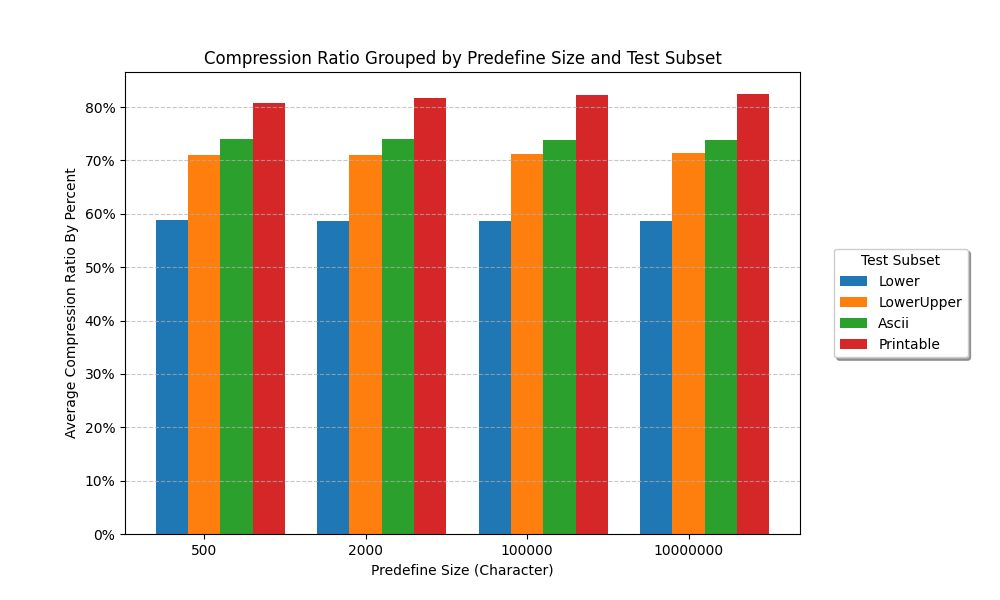
\includegraphics[width=1\textwidth]{figures/project_goals.png}
% 	\caption{Visual Representation of Project Objectives.}
% 	\label{fig:project_goals}
% \end{figure}


\subsection{Scope of the Project}
\subsubsection{In Scope}
The features and functionalities implemented in the final system include:
\begin{itemize}
	\item A secure authentication system for both members and librarians.
	\item Full CRUD (Create, Read, Update, Delete) functionality for the book catalogue.
	\item A complete loan management system.
	\item An interactive console-based user interface (CLI).
	\item Data persistence using local CSV files with a hashing mechanism for integrity.
\end{itemize}

\subsubsection{Out of Scope}
The following features were considered but explicitly excluded:
\begin{itemize}
	\item A Graphical User Interface (GUI).
	\item Integration with a real-time relational database.
	\item Web-based or mobile client interfaces.
\end{itemize}

\subsection{Report Organization}
This report is structured into the following sections to guide the reader from the project's conception to its technical details and conclusion:
\begin{description}
	\item[Section 1 - Introduction:] Outlines the project's purpose, goals, scope, and provides a roadmap for the document.
	\item[Section 2 - System Analysis and Design:] Delves into the high-level design of the application, including the software architecture and the primary UML class diagram.
	\item[Section 3 - Implementation and OOP Principles:] Focuses on the implementation details, providing concrete code examples to demonstrate how the core principles of OOP were applied.
	\item[Section 4 - Software Design Patterns:] Provides a detailed analysis of the design patterns used in the project, explaining their purpose and implementation.
	\item[Section 5 - Service Layer:] Explores the architecture and design of the service layer, detailing its components and their interactions.
	\item[Section 6 - Application Walkthrough:] Demonstrates the system from a user's perspective, using sequence diagrams and screenshots to illustrate key functionalities.
	\item[Section 7 - Conclusion:] Summarizes the project's outcomes, discusses the challenges faced, and proposes directions for future work.
\end{description}